\chapter{新闻事件的主题演化分析方法研究}
第二章,我们介绍了文本分析的常用方法,以及它们在具体场景的应用。然而这些方法并没有考虑文本的产生的时间,在建模时简单认为文本之间是可交换的。显然这样的处理方式不够充分,因为在现实情况中,大部分文本(如,新闻报道,学术文章)都具有时间属性。对同一事物或事件的叙述,随着时间的推移一定会产生变化,而这些变化之间的差异又必然会存在一定的依赖的关系。本章,我们将重点研究新闻语料的特点,并基于此提出一套有效的方法来跟踪新闻事件的主题演化过程。

\section{新闻事件的时序分析}
\subsection{新闻报道的时序分布}
当某一重大新闻事件$E_1$爆发时,通常在较短的时间内,各大媒体都会争相报道,此时关于此事件的报道数量会迅速达到一个峰值$P_1$。随着时间的该事件开始慢慢降温,或者发生了其他更具吸引力的事件$E_2$发生了,那么关于事件$E_1$的报道数量也会回落到一个较小的范围。然而,对于重要的新闻事件,随着时间的发展,不时会有新的信息被披露,每一次信息的披露都会让该事件重新获得上头条的机会,那么新闻的报道数量也就会重新攀升至一个新的峰值$P_2$。如此往复,重大新闻事件往往会经历几个阶段。

如果我们将事件$E_1$每次报道数量达到峰值前后一段时间一起作为一个 \emph{阶段},虽然在这个阶段内新闻的报道数量会非常多,但是实际上大部分的报道内容都非常的相似,因为各家媒体获得信息都差不多。然后,不同的阶段之间,报道的内容会有较大的不同。我们从英国卫报\emph{The Guardian}上分别抓取了以 \emph{Edward Snowden}和\emph{Obamacare}为关键词的新闻报道,Figure.\ref{temporal distribution}表示他们的时序分布。正如我们的猜想,新闻报道的实际时序分布的确包含了多个波峰和波谷。

% BEGIN == 新闻报道的时序分布图
\begin{figure}[htb]
	\subfigure[Edward Snowden]{
		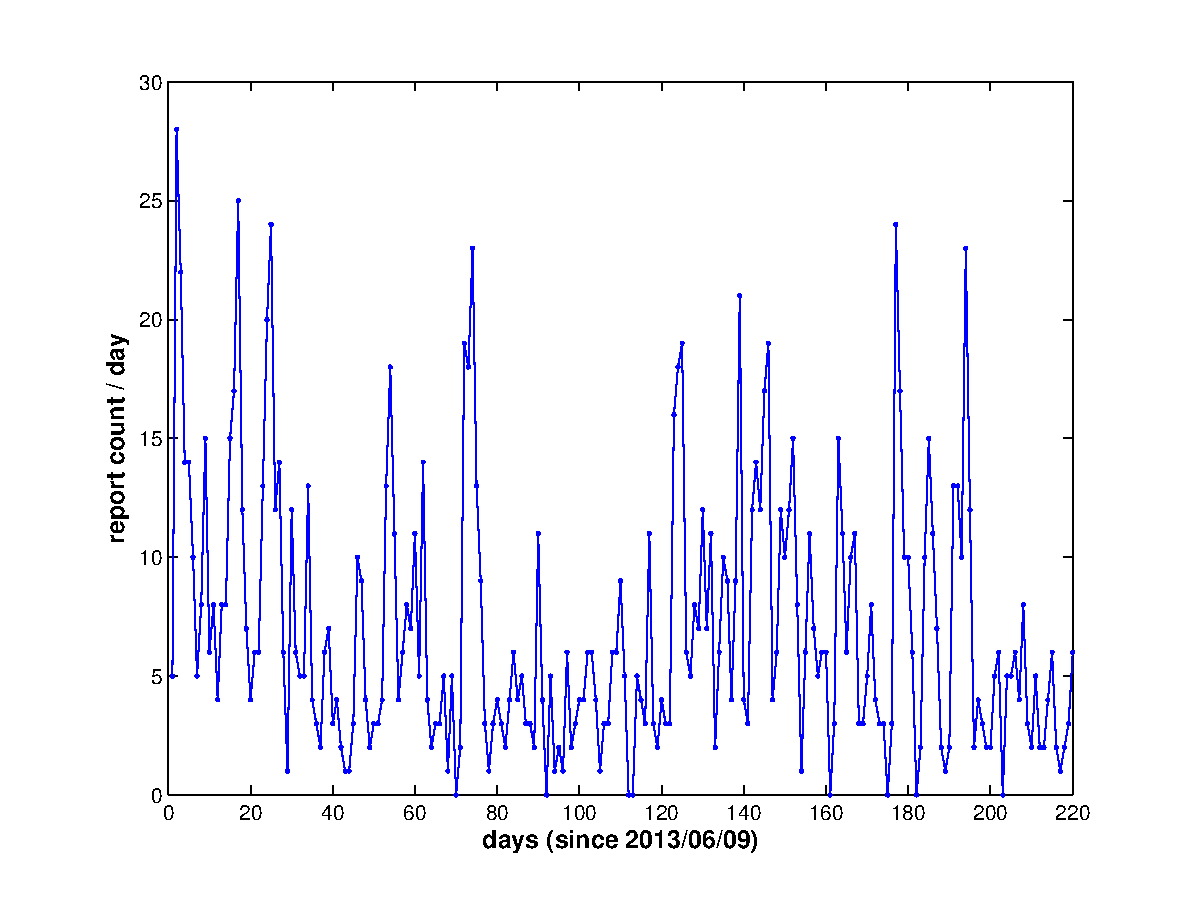
\includegraphics[width=7.5cm]{guardian_snowden}
		\label{temporal distribution:snowden}
	}
	\subfigure[Obamacare]{
		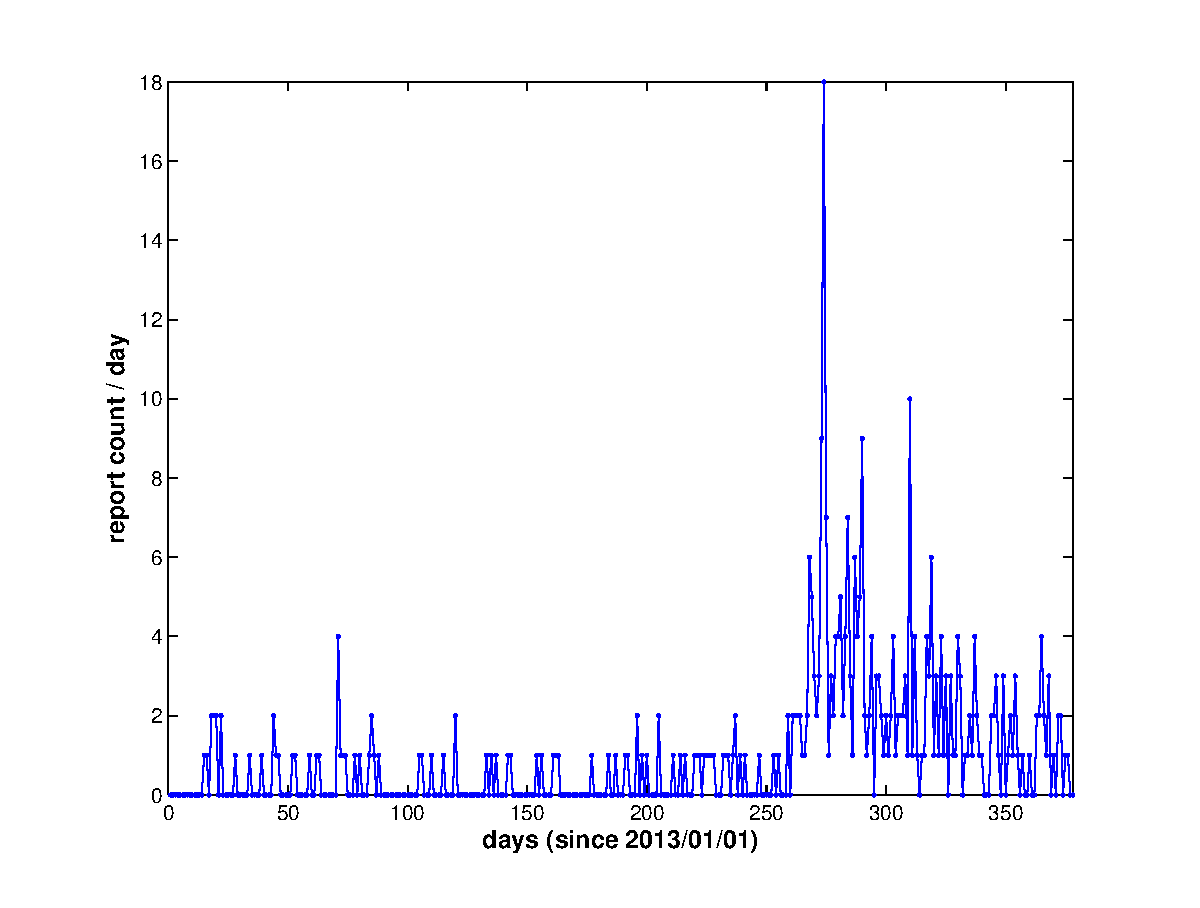
\includegraphics[width=7.5cm]{guardian_obamacare}
		\label{temporal distribution:obamacare}
	}
	\caption{关于"Edward Snowden" 和 "Obamacare" 相关新闻的报道数量时序分布图. X轴表示时间(单位:天),Y轴表示新闻的报道数量(单位:篇)}
	\label{temporal distribution}
\end{figure}
% END == 新闻报道的时序分布图

\subsection{新闻语料的时序划分}
DTM \cite{Blei:2006}是由David Blei等人提出的动态主题模型,